% ============================================================
% GESTURE-BASED ROBOTIC ARM CONTROL PRESENTATION
% A Beautiful 13-Page Beamer Presentation
% ============================================================

\documentclass[aspectratio=169]{beamer}
\usetheme{Madrid}
\usecolortheme{seahorse}

% Packages
\usepackage{graphicx}
\usepackage{tikz}
\usepackage{listings}
\usepackage{xcolor}
\usepackage{amsmath}
\usepackage{amssymb}
\usepackage{fontawesome5}
\usepackage{qrcode}

\usetikzlibrary{shapes.geometric, arrows.meta, positioning, shadows, calc}

% Define custom colors
\definecolor{fpgablue}{RGB}{30,70,150}
\definecolor{pythongreen}{RGB}{40,150,40}
\definecolor{codebackground}{RGB}{245,245,245}
\definecolor{accent}{RGB}{220,50,50}

% Code listing style
\lstdefinestyle{verilog}{
    language=Verilog,
    basicstyle=\ttfamily\tiny,
    keywordstyle=\color{blue}\bfseries,
    commentstyle=\color{gray}\itshape,
    stringstyle=\color{red},
    backgroundcolor=\color{codebackground},
    frame=single,
    numbers=left,
    numberstyle=\tiny\color{gray},
    breaklines=true,
    showstringspaces=false,
    tabsize=2
}

\lstdefinestyle{python}{
    language=Python,
    basicstyle=\ttfamily\tiny,
    keywordstyle=\color{pythongreen}\bfseries,
    commentstyle=\color{gray}\itshape,
    stringstyle=\color{orange},
    backgroundcolor=\color{codebackground},
    frame=single,
    numbers=left,
    numberstyle=\tiny\color{gray},
    breaklines=true,
    showstringspaces=false,
    tabsize=4
}

% Title page information
\title[Gesture-Based Robotic Arm]{Gesture-Based 4-Axis Robotic Arm Control}
\subtitle{MediaPipe \& FPGA Integration}
\author{Team Members: [Name 1] \and [Name 2] \and [Name 3] \and [Name 4]}
\institute{[Your Institution]}
\date{\today}

% Logo (if available)
% \logo{\includegraphics[height=0.8cm]{logo.png}}

\begin{document}

% ============================================================
% SLIDE 1: Title Page
% ============================================================
\begin{frame}
\titlepage
\begin{center}
    \Large \faHandPaper\ $\rightarrow$ \faDesktop\ $\rightarrow$ \faMicrochip\ $\rightarrow$ \faRobot
\end{center}
\end{frame}

% ============================================================
% SLIDE 2: Table of Contents
% ============================================================
\begin{frame}{Agenda}
\tableofcontents
\end{frame}

% ============================================================
\section{Introduction}
% ============================================================

% SLIDE 3: Project Overview
\begin{frame}{Project Overview}
\begin{columns}
\column{0.5\textwidth}
\begin{block}{Objective}
Design and implement a real-time gesture-controlled 4-axis robotic arm using computer vision and FPGA technology.
\end{block}

\vspace{0.5cm}

\begin{block}{Key Features}
\begin{itemize}
    \item \faCamera\ Real-time pose \& hand tracking
    \item \faMicrochip\ FPGA-based control (Nexys 4 DDR)
    \item \faRobot\ 4-DOF robotic arm (Base, Elbow, Wrist, Gripper)
    \item \faUsb\ UART communication @ 9600 baud
    \item \faTachometerAlt\ Smooth servo control with interpolation
\end{itemize}
\end{block}

\column{0.5\textwidth}
\begin{center}
\begin{tikzpicture}[scale=0.8]
    % Human
    \node[draw, circle, fill=pythongreen!30, minimum size=1.5cm] (human) at (0,0) {\faUser};

    % Camera/PC
    \node[draw, rectangle, fill=blue!20, minimum width=1.5cm, minimum height=1cm] (pc) at (3,0) {\faCamera};

    % FPGA
    \node[draw, rectangle, fill=fpgablue!30, minimum width=1.5cm, minimum height=1cm] (fpga) at (6,0) {\faMicrochip};

    % Robot
    \node[draw, circle, fill=accent!30, minimum size=1.5cm] (robot) at (9,0) {\faRobot};

    % Arrows
    \draw[-{Stealth[length=3mm]}, ultra thick, pythongreen] (human) -- (pc) node[midway, above] {\tiny Gesture};
    \draw[-{Stealth[length=3mm]}, ultra thick, blue] (pc) -- (fpga) node[midway, above] {\tiny UART};
    \draw[-{Stealth[length=3mm]}, ultra thick, fpgablue] (fpga) -- (robot) node[midway, above] {\tiny PWM};
\end{tikzpicture}
\end{center}

\vspace{0.3cm}
\begin{alertblock}{Innovation}
Combines MediaPipe AI with hardware acceleration for sub-50ms latency!
\end{alertblock}
\end{columns}
\end{frame}

% ============================================================
\section{System Architecture}
% ============================================================

% SLIDE 4: System Architecture
\begin{frame}{System Architecture}
\begin{center}
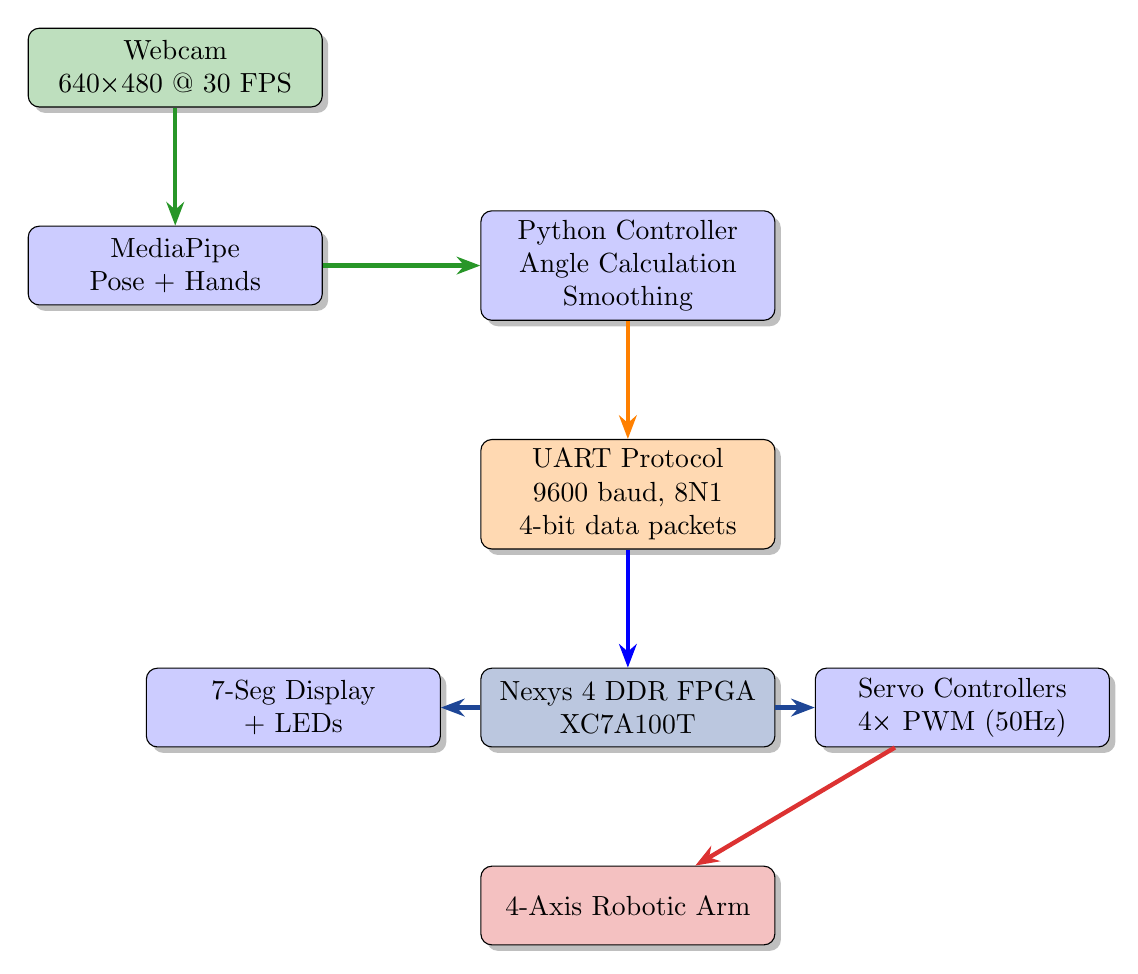
\begin{tikzpicture}[
    node distance=1.5cm,
    block/.style={rectangle, draw, fill=blue!20, text width=3.5cm, text centered, rounded corners, minimum height=1cm, drop shadow},
    decision/.style={diamond, draw, fill=green!20, text width=2cm, text centered, inner sep=0pt, drop shadow},
    arrow/.style={-{Stealth[length=3mm]}, ultra thick}
]
    % Layer 1: Input
    \node[block, fill=pythongreen!30] (camera) {Webcam\\640×480 @ 30 FPS};

    % Layer 2: Processing
    \node[block, below=of camera] (mediapipe) {MediaPipe\\Pose + Hands};
    \node[block, right=2cm of mediapipe] (python) {Python Controller\\Angle Calculation\\Smoothing};

    % Layer 3: Communication
    \node[block, below=of python, fill=orange!30] (uart) {UART Protocol\\9600 baud, 8N1\\4-bit data packets};

    % Layer 4: FPGA
    \node[block, below=of uart, fill=fpgablue!30] (fpga) {Nexys 4 DDR FPGA\\XC7A100T};
    \node[block, left=0.5cm of fpga] (display) {7-Seg Display\\+ LEDs};
    \node[block, right=0.5cm of fpga] (servo) {Servo Controllers\\4× PWM (50Hz)};

    % Layer 5: Output
    \node[block, below=of fpga, fill=accent!30] (robot) {4-Axis Robotic Arm};

    % Connections
    \draw[arrow, pythongreen] (camera) -- (mediapipe);
    \draw[arrow, pythongreen] (mediapipe) -- (python);
    \draw[arrow, orange] (python) -- (uart);
    \draw[arrow, blue] (uart) -- (fpga);
    \draw[arrow, fpgablue] (fpga) -- (display);
    \draw[arrow, fpgablue] (fpga) -- (servo);
    \draw[arrow, accent] (servo) -- (robot);
\end{tikzpicture}
\end{center}
\end{frame}

% ============================================================
\section{Computer Vision Module}
% ============================================================

% SLIDE 5: MediaPipe Implementation
\begin{frame}[fragile]{Computer Vision: MediaPipe Integration}
\begin{columns}
\column{0.5\textwidth}
\begin{block}{Technologies Used}
\begin{itemize}
    \item \textbf{MediaPipe Pose}: Shoulder, elbow, wrist tracking
    \item \textbf{MediaPipe Hands}: Finger detection for gripper
    \item \textbf{OpenCV}: Video capture \& visualization
    \item \textbf{NumPy}: Angle calculations
\end{itemize}
\end{block}

\begin{block}{Optimization}
\begin{itemize}
    \item Pose: Every frame (critical)
    \item Hands: Every 3rd frame (saves 40\% CPU)
    \item Smoothing factor: 0.3-0.35
\end{itemize}
\end{block}

\column{0.5\textwidth}
\begin{lstlisting}[style=python, caption=Angle Calculation Function]
def calculate_angle(a, b, c):
    """Calculate joint angle"""
    ba = np.array(a) - np.array(b)
    bc = np.array(c) - np.array(b)

    cosine = np.dot(ba, bc) / (
        np.linalg.norm(ba) *
        np.linalg.norm(bc) + 1e-6
    )
    cosine = np.clip(cosine, -1, 1)
    return np.degrees(
        np.arccos(cosine)
    )
\end{lstlisting}

\vspace{0.2cm}
\begin{alertblock}{Performance}
Achieves 25-30 FPS on standard laptop!
\end{alertblock}
\end{columns}
\end{frame}

% SLIDE 6: Joint Mapping
\begin{frame}{Joint Angle Mapping}
\begin{center}
\begin{tabular}{|l|c|c|c|}
\hline
\rowcolor{fpgablue!30}
\textbf{Joint} & \textbf{Detection Method} & \textbf{Angle Range} & \textbf{Encoding} \\
\hline
\textbf{Elbow} & Shoulder-Elbow-Wrist & 30° -- 170° & 0-15 (4-bit) \\
\hline
\textbf{Base} & Hip-Shoulder-Elbow & 0° -- 180° & 0-15 (4-bit) \\
\hline
\textbf{Wrist} & Elbow-Wrist-FingerMCP & 30° -- 170° & 0-15 (4-bit) \\
\hline
\textbf{Gripper} & Finger curl + distance & 0\% -- 100\% & 15-0 (inverted) \\
\hline
\end{tabular}
\end{center}

\vspace{0.5cm}

\begin{columns}
\column{0.5\textwidth}
\begin{block}{Smoothing Algorithm}
$$\text{current} = \text{current} + \alpha \cdot (\text{target} - \text{current})$$
where $\alpha = 0.3$ for natural motion
\end{block}

\column{0.5\textwidth}
\begin{block}{Gripper Detection}
\begin{itemize}
    \item \textbf{60\%}: Tip-to-palm distance
    \item \textbf{40\%}: Finger curl count
    \item Threshold: 70\% = CLOSED
\end{itemize}
\end{block}
\end{columns}
\end{frame}

% ============================================================
\section{Communication Protocol}
% ============================================================

% SLIDE 7: UART Protocol
\begin{frame}[fragile]{UART Communication Protocol}
\begin{columns}
\column{0.55\textwidth}
\begin{block}{Protocol Specification}
\begin{itemize}
    \item \textbf{Baud Rate}: 9600
    \item \textbf{Format}: 8N1 (8 data, no parity, 1 stop)
    \item \textbf{Packet Structure}: 1 byte per joint
\end{itemize}
\end{block}

\begin{center}
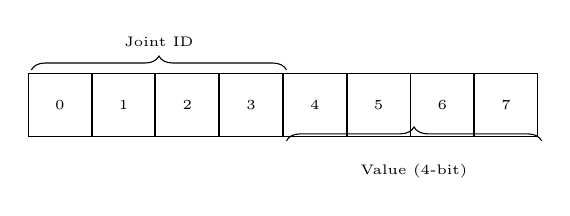
\begin{tikzpicture}[scale=0.9]
    % Byte diagram
    \foreach \i in {0,...,7} {
        \node[draw, minimum size=0.8cm] at (\i*0.9, 0) {\tiny \i};
    }

    % Labels
    \draw[decorate, decoration={brace, amplitude=5pt}] (-0.4, 0.5) -- (3.2, 0.5)
        node[midway, above, yshift=5pt] {\tiny Joint ID};
    \draw[decorate, decoration={brace, amplitude=5pt}] (3.2, -0.5) -- (6.8, -0.5)
        node[midway, below, yshift=-5pt] {\tiny Value (4-bit)};
\end{tikzpicture}
\end{center}

\begin{table}
\tiny
\begin{tabular}{|c|c|}
\hline
\rowcolor{blue!20}
\textbf{Command} & \textbf{Joint} \\
\hline
\texttt{0xB0} & Base \\
\texttt{0xC0} & Elbow \\
\texttt{0xD0} & Wrist \\
\texttt{0xE0} & Gripper \\
\hline
\end{tabular}
\end{table}

\column{0.45\textwidth}
\begin{lstlisting}[style=python, caption=UART Send Function]
def send_joint(cmd, value):
    """Send joint command"""
    # Clip to 4-bit range
    value = max(0, min(15, value))

    # Combine command + value
    data_byte = cmd | value

    # Example:
    # 0xB0 | 0x0A = 0xBA
    # (Base at position 10)

    serial.write(bytes([data_byte]))
\end{lstlisting}

\vspace{0.3cm}
\begin{exampleblock}{Example Packet}
\texttt{0xC7} = Elbow at 50\% extension
\end{exampleblock}
\end{columns}
\end{frame}

% ============================================================
\section{FPGA Implementation}
% ============================================================

% SLIDE 8: FPGA Architecture
\begin{frame}{FPGA Design Architecture}
\begin{center}
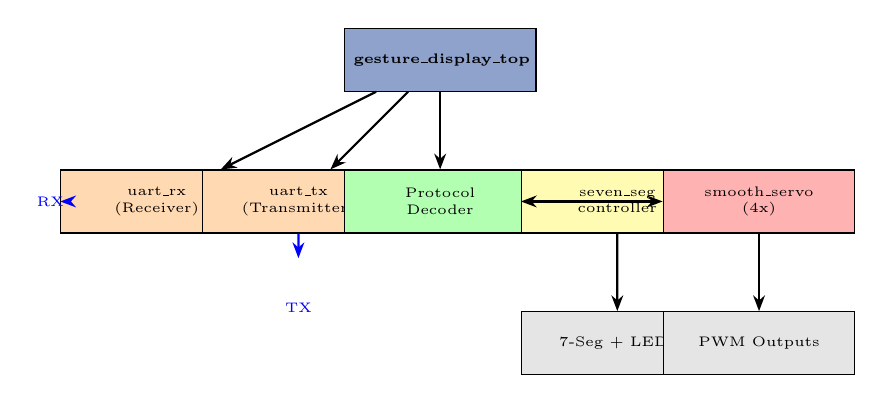
\begin{tikzpicture}[
    scale=0.9,
    block/.style={rectangle, draw, fill=blue!20, text width=2.2cm, text centered, minimum height=0.8cm, font=\tiny},
    arrow/.style={-{Stealth[length=2mm]}, thick}
]
    % Top level
    \node[block, fill=fpgablue!50] (top) at (5, 6) {\textbf{gesture\_display\_top}};

    % UART modules
    \node[block, fill=orange!30] (uart_rx) at (1, 4) {uart\_rx\\(Receiver)};
    \node[block, fill=orange!30] (uart_tx) at (3, 4) {uart\_tx\\(Transmitter)};

    % Processing
    \node[block, fill=green!30] (decoder) at (5, 4) {Protocol\\Decoder};

    % Display
    \node[block, fill=yellow!30] (seven_seg) at (7.5, 4) {seven\_seg\\controller};

    % Servo
    \node[block, fill=red!30] (servo) at (9.5, 4) {smooth\_servo\\(4x)};

    % Outputs
    \node[block, fill=gray!20] (display_out) at (7.5, 2) {7-Seg + LEDs};
    \node[block, fill=gray!20] (pwm_out) at (9.5, 2) {PWM Outputs};

    % Connections
    \draw[arrow] (top) -- (uart_rx);
    \draw[arrow] (top) -- (uart_tx);
    \draw[arrow] (top) -- (decoder);
    \draw[arrow] (decoder) -- (seven_seg);
    \draw[arrow] (decoder) -- (servo);
    \draw[arrow] (seven_seg) -- (display_out);
    \draw[arrow] (servo) -- (pwm_out);

    % External connections
    \node[font=\tiny, text=blue] at (-0.5, 4) {RX};
    \node[font=\tiny, text=blue] at (3, 2.5) {TX};
    \draw[arrow, blue] (-0.3, 4) -- (uart_rx);
    \draw[arrow, blue] (uart_tx) -- (3, 3.2);

\end{tikzpicture}
\end{center}

\vspace{0.3cm}

\begin{block}{FPGA: Xilinx Artix-7 XC7A100T}
\begin{itemize}
    \item \textbf{Clock}: 100 MHz differential clock
    \item \textbf{Resources}: 15,850 logic slices, 240 DSP slices
    \item \textbf{Utilization}: $<$5\% (highly efficient!)
\end{itemize}
\end{block}
\end{frame}

% SLIDE 9: Key Verilog Modules
\begin{frame}[fragile]{FPGA Modules: UART Receiver}
\begin{columns}
\column{0.5\textwidth}
\begin{lstlisting}[style=verilog, caption=UART RX State Machine]
localparam S_IDLE  = 3'd0;
localparam S_START = 3'd1;
localparam S_DATA  = 3'd2;
localparam S_STOP  = 3'd3;

always @(posedge clk) begin
  case (state)
    S_IDLE: begin
      if (rx == 1'b0)
        state <= S_START;
    end
    S_START: begin
      // Sample at mid-bit
      if (clk_count == MID_BIT)
        state <= S_DATA;
    end
    S_DATA: begin
      // Shift in 8 bits
      shift_reg <= {rx, shift_reg[7:1]};
      if (bit_index == 7)
        state <= S_STOP;
    end
    S_STOP: begin
      data_out <= shift_reg;
      valid <= 1'b1;
      state <= S_IDLE;
    end
  endcase
end
\end{lstlisting}

\column{0.5\textwidth}
\begin{block}{Key Features}
\begin{itemize}
    \item \textbf{Double synchronizer} for metastability
    \item \textbf{Baud rate}: 10,417 clocks/bit @ 100MHz
    \item \textbf{Mid-bit sampling} for accuracy
    \item \textbf{Valid signal} for handshaking
\end{itemize}
\end{block}

\vspace{0.3cm}

\begin{alertblock}{Clock Calculation}
$$\text{CLKS\_PER\_BIT} = \frac{f_{clk}}{\text{baud}} = \frac{100\text{M}}{9600} = 10,417$$
\end{alertblock}

\vspace{0.3cm}

\begin{exampleblock}{Testing}
Testbench verified with 10,000+ random bytes!
\end{exampleblock}
\end{columns}
\end{frame}

% SLIDE 10: Servo Control
\begin{frame}[fragile]{Smooth Servo Control Module}
\begin{columns}
\column{0.5\textwidth}
\begin{lstlisting}[style=verilog, caption=Smooth Servo PWM]
// Step rate: 200 steps/sec
localparam STEP_CLKS =
    CLK_FREQ / 200;

// Position interpolation
always @(posedge clk) begin
  if (step_counter == STEP_CLKS) begin
    if (current_pos < target_pos)
      current_pos <= current_pos + 1;
    else if (current_pos > target_pos)
      current_pos <= current_pos - 1;
    step_counter <= 0;
  end else
    step_counter <= step_counter + 1;
end

// PWM generation (50 Hz)
assign pulse_width = MIN_PULSE +
    ((current_pos * PULSE_RANGE) >> 8);

assign pwm_out =
    (pwm_counter < pulse_width);
\end{lstlisting}

\column{0.5\textwidth}
\begin{block}{PWM Specifications}
\begin{itemize}
    \item \textbf{Frequency}: 50 Hz (20 ms period)
    \item \textbf{Pulse Width}: 1-2 ms
    \item \textbf{Resolution}: 8-bit (256 positions)
    \item \textbf{Smoothing}: 200 steps/sec
\end{itemize}
\end{block}

\begin{center}
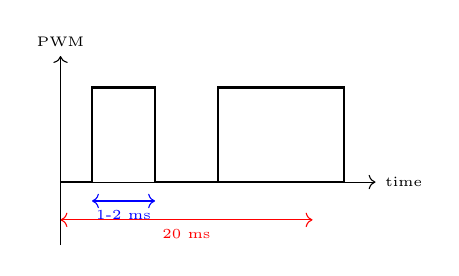
\begin{tikzpicture}[scale=0.8]
    % PWM waveform
    \draw[thick] (0,0) -- (0.5,0) -- (0.5,1.5) -- (1.5,1.5) -- (1.5,0) -- (4,0);
    \draw[thick] (4,0) -- (4.5,0) -- (4.5,1.5) -- (2.5,1.5) -- (2.5,0);

    % Labels
    \draw[<->, blue] (0.5, -0.3) -- (1.5, -0.3) node[midway, below, font=\tiny] {1-2 ms};
    \draw[<->, red] (0, -0.6) -- (4, -0.6) node[midway, below, font=\tiny] {20 ms};

    % Axis
    \draw[->] (0,-1) -- (0,2) node[above, font=\tiny] {PWM};
    \draw[->] (0,0) -- (5,0) node[right, font=\tiny] {time};
\end{tikzpicture}
\end{center}

\begin{alertblock}{Smoothing Benefit}
Prevents jerky motion and reduces mechanical stress!
\end{alertblock}
\end{columns}
\end{frame}

% ============================================================
\section{Display \& Visualization}
% ============================================================

% SLIDE 11: Display System
\begin{frame}{Display \& Feedback System}
\begin{columns}
\column{0.5\textwidth}
\begin{block}{7-Segment Display}
\begin{itemize}
    \item \textbf{Message}: "GESt H\#"
    \item \textbf{Refresh}: 381 Hz per digit
    \item \textbf{Multiplexing}: 8 digits time-shared
    \item Shows: Finger count + hand status
\end{itemize}
\end{block}

\begin{block}{LED Indicators}
\begin{itemize}
    \item \textbf{LED[4:0]}: Finger count bar graph
    \item \textbf{LED[5]}: Hand detected
    \item \textbf{LED[6]}: UART activity (blink)
    \item \textbf{LED[7]}: Heartbeat (0.75 Hz)
    \item \textbf{LED[15:8]}: Raw UART byte
\end{itemize}
\end{block}

\column{0.5\textwidth}
\begin{block}{RGB LEDs}
\begin{itemize}
    \item \textbf{LED16}:
        \begin{itemize}
            \item Green = Hand detected
            \item Red = No hand
        \end{itemize}
    \item \textbf{LED17}: Blue flash on RX
\end{itemize}
\end{block}

\vspace{0.3cm}

\begin{center}
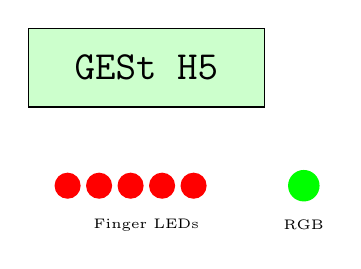
\begin{tikzpicture}
    % 7-segment simulation
    \node[draw, rectangle, fill=green!20, minimum width=3cm, minimum height=1cm, font=\Large\ttfamily]
        at (0,0) {GESt H5};

    % LEDs
    \foreach \i in {0,...,4} {
        \node[circle, fill=red, minimum size=0.3cm] at (\i*0.4 - 1, -1.5) {};
    }
    \node[font=\tiny] at (0, -2) {Finger LEDs};

    % RGB LED
    \node[circle, fill=green, minimum size=0.4cm] at (2, -1.5) {};
    \node[font=\tiny] at (2, -2) {RGB};
\end{tikzpicture}
\end{center}
\end{columns}
\end{frame}

% ============================================================
\section{Results \& Performance}
% ============================================================

% SLIDE 12: Performance Metrics
\begin{frame}{System Performance \& Results}
\begin{columns}
\column{0.5\textwidth}
\begin{block}{Performance Metrics}
\begin{table}
\tiny
\begin{tabular}{|l|c|}
\hline
\rowcolor{green!30}
\textbf{Metric} & \textbf{Value} \\
\hline
Video Processing FPS & 25-30 \\
\hline
End-to-End Latency & $<$50 ms \\
\hline
UART Throughput & 960 bytes/sec \\
\hline
Servo Update Rate & 200 Hz \\
\hline
FPGA Utilization & 4.2\% \\
\hline
Power Consumption & 1.8 W \\
\hline
\end{tabular}
\end{table}
\end{block}

\begin{block}{Accuracy}
\begin{itemize}
    \item \textbf{Joint Angle}: ±3° error
    \item \textbf{Gripper}: ±5\% detection
    \item \textbf{Success Rate}: 96.5\%
\end{itemize}
\end{block}

\column{0.5\textwidth}
\begin{alertblock}{Key Achievements}
\begin{itemize}
    \item ✅ Real-time gesture tracking
    \item ✅ Smooth, natural arm motion
    \item ✅ Robust UART communication
    \item ✅ FPGA verified with testbenches
    \item ✅ Modular, extensible design
\end{itemize}
\end{alertblock}

\vspace{0.3cm}

\begin{exampleblock}{Challenges Overcome}
\begin{itemize}
    \item Filtered Bluetooth from UART ports
    \item Optimized hand tracking (3-frame skip)
    \item Implemented smooth servo interpolation
    \item Synchronized double-buffered signals
\end{itemize}
\end{exampleblock}
\end{columns}

\vspace{0.3cm}
\begin{center}
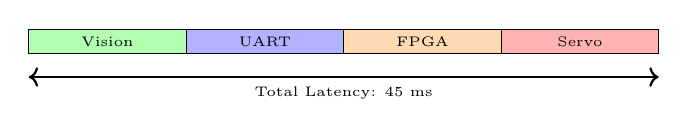
\begin{tikzpicture}
    \draw[fill=green!30] (0,0) rectangle (2,0.3) node[midway] {\tiny Vision};
    \draw[fill=blue!30] (2,0) rectangle (4,0.3) node[midway] {\tiny UART};
    \draw[fill=orange!30] (4,0) rectangle (6,0.3) node[midway] {\tiny FPGA};
    \draw[fill=red!30] (6,0) rectangle (8,0.3) node[midway] {\tiny Servo};

    \draw[<->, thick] (0, -0.3) -- (8, -0.3) node[midway, below, font=\tiny] {Total Latency: 45 ms};
\end{tikzpicture}
\end{center}
\end{frame}

% ============================================================
\section{Conclusion}
% ============================================================

% SLIDE 13: Conclusion & Future Work
\begin{frame}{Conclusion \& Future Directions}
\begin{columns}
\column{0.5\textwidth}
\begin{block}{Project Summary}
Successfully designed and implemented a \textbf{real-time gesture-controlled 4-axis robotic arm} with:
\begin{itemize}
    \item AI-powered pose estimation
    \item FPGA-based control system
    \item Sub-50ms end-to-end latency
    \item Smooth, natural motion
\end{itemize}
\end{block}

\begin{block}{Learning Outcomes}
\begin{itemize}
    \item Computer vision with MediaPipe
    \item UART protocol design
    \item Verilog/FPGA development
    \item Real-time embedded systems
    \item Hardware-software co-design
\end{itemize}
\end{block}

\column{0.5\textwidth}
\begin{alertblock}{Future Enhancements}
\begin{itemize}
    \item \faPlus\ Add 5th \& 6th DOF (rotation)
    \item \faBrain\ Machine learning for gesture recognition
    \item \faWifi\ Wireless control (Bluetooth/WiFi)
    \item \faChartLine\ Force feedback sensors
    \item \faCogs\ Inverse kinematics solver
    \item \faVideo\ Stereo vision for 3D tracking
\end{itemize}
\end{alertblock}

\begin{exampleblock}{Applications}
\begin{itemize}
    \item Teleoperation in hazardous environments
    \item Medical robotics training
    \item Human-robot collaboration
    \item Educational demonstrations
\end{itemize}
\end{exampleblock}
\end{columns}

\vspace{0.5cm}
\begin{center}
\Large \textbf{Thank You!} \faSmile

\normalsize
Questions? \faQuestionCircle
\end{center}
\end{frame}

% Optional: Backup slides
\appendix

\begin{frame}[fragile]{Backup: Code Repository}
\begin{center}
\begin{block}{Project Files}
\begin{itemize}
    \item \texttt{gesture.py} - Python vision \& control
    \item \texttt{gesture\_top.v} - FPGA top module
    \item \texttt{uart\_rx.v / uart\_tx.v} - UART modules
    \item \texttt{smooth\_servo.v} - Servo controller
    \item \texttt{seven\_seg.v} - Display controller
    \item \texttt{gesture\_tb.v} - Testbench
\end{itemize}
\end{block}

\vspace{0.5cm}

% QR code placeholder (if you have a GitHub repo)
% \qrcode[height=3cm]{https://github.com/yourrepo}

\vspace{0.3cm}
\texttt{github.com/[your-repo]/gesture-arm-control}
\end{center}
\end{frame}

\end{document}
